\documentclass{beamer}					%printtaukseen [handout]
\usetheme{Frankfurt}
\usecolortheme{dove}

%\usepackage{pgfpages}							%printtaukseen
%\pgfpagesuselayout{2 on 1}[a4paper,border shrink=5mm]	%printtaukseen

\usepackage[T1]{fontenc}
\usepackage[utf8]{inputenc}
\usepackage{lmodern}
%\usepackage{natbib}							%for citations in Harvard style
\usepackage{xcolor}
\usepackage{amsmath}
\usepackage{mathtools}
\usepackage{amsfonts}
\usepackage{amssymb}
\usepackage{xfrac}
\usepackage[british]{babel}
\usepackage{cleveref}						%for multiple refs in one ref
\renewcommand*\familydefault{\ttdefault} %% Only if the base font of the document is to be typewriter style
\usepackage{courier}
\usepackage{booktabs}
\usepackage[backend=biber,citestyle=authoryear,bibstyle=authoryear]{biblatex}
\addbibresource{references.bib}
\usepackage{csquotes} % for proper quotation marks
\usepackage{textpos}

\DeclareMathOperator*{\E}{\mathbb{E}}				% Expectation symbol



%%%%% PATHS %%%%%

\graphicspath{{./plotit/}}
\DeclareGraphicsExtensions{.png,.pdf,.eps,.jpg}
%\addbibresource{refs.bib} %for citations

%%%% CUSTOMIZATION OF THE TEMPLATE %%%%%

\useinnertheme{rectangles} %rectangle bullets etc
\beamertemplatenavigationsymbolsempty	%no navigation bar
\setbeamercovered{transparent}		%future bullet points transparent 
\setbeamertemplate{frametitle}[default][colsep=-4bp,rounded=false,shadow=false] %no shadows
\definecolor{dark-gray}{gray}{0.80} %color for the navigation squares

%%%% FOOTLINE CUSTOMIZATION %%%%%

\setbeamercolor{section in head/foot}{fg=black, bg=white}
\makeatletter
\setbeamertemplate{footline}
{
	\leavevmode%
	\hbox{%
	\begin{beamercolorbox}[wd=.333333\paperwidth,ht=2.25ex,dp=1ex,center]{section in head/foot}%
		%\usebeamerfont{author in head/foot}\insertshortauthor~~
		%\beamer@ifempty{\insertshortinstitute}{}{(\insertshortinstitute)}
	\end{beamercolorbox}%
	\begin{beamercolorbox}[wd=.333333\paperwidth,ht=2.25ex,dp=1ex,center]{section in head/foot}%
 		%\usebeamerfont{title in head/foot}\insertshorttitle
	\end{beamercolorbox}%
	\begin{beamercolorbox}[wd=.333333\paperwidth,ht=2.25ex,dp=1ex,right]{section in head/foot}%
		%\usebeamerfont{date in head/foot}\insertshortdate{}\hspace*{2em}
		\insertframenumber{} / \inserttotalframenumber\hspace*{2ex} 
	\end{beamercolorbox}
    }%
	\vskip0pt%
}

%%%% HEADER CUSTOMIZATION %%%%%


\setbeamertemplate{mini frame}
{%
  \begin{pgfpicture}{0pt}{0pt}{.1cm}{.1cm}
    \pgfpathrectangle{\pgfpointorigin}{\pgfpoint{\the\beamer@boxsize}{\the\beamer@boxsize}}
    \pgfusepath{fill,stroke}
  \end{pgfpicture}%
}

\def\slideentry#1#2#3#4#5#6{%
  %section number, subsection number, slide number, first/last frame, page number, part number
  \ifnum#6=\c@part\ifnum#2>0\ifnum#3>0%
    \ifbeamer@compress%
      \advance\beamer@xpos by1\relax%
    \else%
      \beamer@xpos=#3\relax%
      \beamer@ypos=#2\relax%
    \fi%
  \hbox to 2pt{%
    \beamer@tempdim=-\beamer@vboxoffset%
    \advance\beamer@tempdim by-\beamer@boxsize%
    \multiply\beamer@tempdim by\beamer@ypos%
    \advance\beamer@tempdim by -.05cm%
    \raise\beamer@tempdim\hbox{%
      \beamer@tempdim=\beamer@boxsize%
      \multiply\beamer@tempdim by\beamer@xpos%
      \advance\beamer@tempdim by -\beamer@boxsize%
      \advance\beamer@tempdim by 1pt%
      \kern\beamer@tempdim
      \global\beamer@section@min@dim\beamer@tempdim
      \hbox{\beamer@link(#4){%
          \usebeamerfont{mini frame}%
          \ifnum\c@section>#1%
            \color{dark-gray}%
          \else%
            \ifnum\c@section=#1%
              \ifnum\c@subsection>#2%
                \color{dark-gray}%
              \else%
                \ifnum\c@subsection=#2%
                  \ifnum\c@subsectionslide>#3%
                    \color{dark-gray}%
                  \else%
                    \color{fg}%
                  \fi%
                \else%
                  \color{dark-gray}%
                \fi%
              \fi%
            \else%
              \color{dark-gray}%
            \fi%
          \fi%
          \usebeamertemplate{mini frame}%
        }}}\hskip-10cm plus 1fil%
  }\fi\fi%
  \else%
  \fakeslideentry{#1}{#2}{#3}{#4}{#5}{#6}%
  \fi\ignorespaces
  }
  
%%%% SOME BUG %%%%%

\def\pdftex@driver{pdftex.def}
\ifx\Gin@driver\pdftex@driver
  \def\pgfsys@color@unstacked#1{%
    \pdfliteral{\csname\string\color@#1\endcsname}%
  }
\fi

\makeatother



%%%%% INFORMATION ABOUT THE DOCUMENT %%%%%

\title[Thesis presentation]{Efficient Evidence Accumulation Clustering for large datasets / big data}

\author[Silva]{Diogo Alexandre Oliveira Silva \\ \tiny ALFAL / ENGEL}

\institute[AFA/IST]{
Academia da For\c{c}a A\'erea / Instituto Superior T\'ecnico \\
% \medskip
% %\textit{john@smith.com} % Your email address
% \vspace{2mm}
% \tiny \scalebox{1.2}{\textbf{J\'uri}}\\
% \vspace{2mm}
% \begin{tabular}{ll}
%  \tiny Presidente:						& \tiny Prof. Dr. Jo\~ao da Silva Sequeira\\ 
%  \tiny Orientador:						& \tiny Prof. Dr. Ana Lu\'sa Nobre Fred \\ 
%  \tiny Vogais:	 						& \tiny BGEN/ENGEL Luis Filipe Basto Dam\'asio\\
% 										& \tiny TCOR/ENGEL Ana Paula da Silva Jorge\\	
%  	 									& \tiny Prof. Dr. Pedro Filipe Zeferino Tom\'as\\
% \end{tabular}
}

\titlegraphic{\includegraphics[scale=0.06]{afa}\hfill%\hspace*{4.75cm}~%
   \includegraphics[scale=0.14]{IST_A_CMYK_POS}
}

\date{November, 2015}

					  
%%%%% ACTUAL DOCUMENT PAGES %%%%%					  

\begin{document}


\begin{frame}[plain]

%Instirutions symbols
%\begin{flushleft}
%\includegraphics[bb=4cm 11cm 0cm 0cm,scale=0.14]{IST_A_CMYK_POS}
%\includegraphics[bb=-186cm 15cm 0cm 0cm,scale=0.06]{afa}

% \includegraphics[bb=4cm 13cm 0cm 0cm,scale=0.14]{IST_A_CMYK_POS}
% \includegraphics[bb=-180cm 16cm 0cm 0cm,scale=0.05]{afa}
%\end{flushleft}

% \begin{textblock}{20}(0,0)
%       \includegraphics[scale=0.14]{IST_A_CMYK_POS}
% \end{textblock}

% \begin{picture}(0,0)
% \put(100,100){\hbox{\includegraphics[scale=0.14]{IST_A_CMYK_POS}}}
% \end{picture} 

% \begin{figure}
% \centering
% \begin{minipage}{.5\textwidth}
%   \centering
%   \includegraphics[scale=0.14]{IST_A_CMYK_POS}
% \end{minipage}%
% \hfill
% \begin{minipage}{.5\textwidth}
%   \centering
%   \includegraphics[scale=0.06]{afa}
% \end{minipage}
% \end{figure}

\titlepage

\end{frame}

%--------------------------------------------%
%    OVERVIEW 
%--------------------------------------------%

\begin{frame}
\frametitle{Contents} % Table of contents slide, comment this block out to remove it
\footnotesize \tableofcontents % Throughout your presentation, if you choose to use \section{} and \subsection{} commands, these will automatically be printed on this slide as an overview of your presentation
\end{frame}

          


%!TEX root = thesis.tex

\section{Introduction}
\label{intro}

\subsection{The problem of clustering}


%TODO
% problems under Big Data paradihm
% typical challenges with Big Data
% why EAC?
% combination of both
\subsection{Motivation}
The scope of the thesis is Big Data and Cluster Ensembles.

Success of EAC clustering on hard data sets.

Interesting problems from big data.

Combining the two.

\subsection{Challenges and Motivation}

\subsection{Goals and Contribution}

This dissertation aims to research and extend the state of the art of ensemble clustering, in what concerns the method of Evidence Accumulation Clustering and its application in large datasets, while also accessing alternative algorithmic solutions and parallelization techniques. The goal is to understand EAC's suitability for large datasets and find ways to respond to the challenges that that entails (speed and memory). In particular, efficient parallel version for the \gls{gpu} of different parts of the method.

Throughout this dissertation, various clustering techniques are reviewed, implemented and tested. 

\subsection{Objectives}
The main objectives for this work are:
\begin{itemize}

\item Review quantum inspired clustering methods

\item Study possibility of integration of quantum inspired methods in EAC

\item Review of scalability of EAC

\item Review methods and techniques designed for processing large datasets

\item Review of acceleration techniques for large datasets

\item Review of the General Purpose computing in Graphics Processing Units paradigm

\item Study possibility of integration of GPGPU in EAC

\item Devise strategies to reduce complexity of EAC

\item \textbf{Application of Evidence Accumulation Clustering in Big Data}

\item Validation of Big Data EAC on real data (ECG for emotional state discovery and/or discovery of natural groups)
\end{itemize}

\subsection{Outline}

Explain briefly the work done

The scope of the thesis is Big Data and Cluster Ensembles. A main requirement in this context is to have fast clustering techniques. This may be accomplished in two ways: algorithmically or with parallelization techniques. The former deals with finding faster solutions while the later takes existing solutions and optimizes them with execution speed in mind.

The initial research was under the algorithmic path. More specifically, exploring quantum inspired clustering algorithms. The findings of this exploration revealed this algorithms to be a poor match for integration in EAC and turned the focus of the research to parallelization techniques. Two main paradigms of parallelization were found appropriate: GPGPU and distributed (among a cluster of workstations). While the first is a readily available resource in common machines, the second is able to address problems dealing with larger datasets.


%--------------------------------------------%
%--------------------------------------------%
%    PROPOSED SOLUTION 
%--------------------------------------------%
%--------------------------------------------%

\section{Proposed solution}

\subsection{Overview}

% FRAME: OVERVIEW OF PROPOSED SOLUTION
\begin{frame}{Proposed solution: overview}
\begin{figure}[hbt!]
  \centering
  \includegraphics[width=0.8\columnwidth]{{{diagram_proposed_solutions}}}
  %\caption{[1] A. N. L. Fred and A. K. Jain, “Combining multiple clusterings using evidence accumulation,” IEEE Transactions on Pattern Analysis and Machine Intelligence, vol. 27}
  \label{fig:eac kmin evo}
\end{figure}

\end{frame}

\begin{frame}{Proposed solution: final}
\begin{figure}[hbt!]
  \centering
  \includegraphics[width=1.0\columnwidth]{{{diagram_proposed_solutions_BAD}}}
  %\caption{[1] A. N. L. Fred and A. K. Jain, “Combining multiple clusterings using evidence accumulation,” IEEE Transactions on Pattern Analysis and Machine Intelligence, vol. 27}
  \label{fig:eac kmin evo}
\end{figure}

\end{frame}

%--------------------------------------------%
%    PRODUCTION PHASE
%--------------------------------------------%
\subsection{Production}

\begin{frame}{Optimizing production of ensemble}

\begin{itemize}

\item K-Means is simple and has been used with EAC before with success.

\item K-Means:

  \begin{itemize}
  \item \textbf{labelling}: find the closest centroid to each data pattern
  % $$
  % l_i = arg \: \min_k \;d(x_i, c_k)
  % $$
  \item \textbf{update}: new centroids are the mean of the assigned patterns
  % $$
  % c_k = \sum_{i : l_i = k} x_i
  % $$

  \end{itemize}

\item Number of clusters from interval [$K_{min},K_{max}$]

\item Optimization through parallelization in GPU.

\end{itemize}

\end{frame}



\begin{frame}{GPGPU K-Means}

\begin{itemize}

\item CUDA GPGPU

  \begin{itemize}
  \item Hundreds of processors

  \item \emph{Single instruction multiple thread} approach

  \item Shared memory between threads

  \end{itemize}
\end{itemize}

\end{frame}



\begin{frame}{GPU K-Means}

\begin{itemize}

% \item CUDA GPGPU
\item GPU

  \begin{itemize}
  \item Hundreds of processors

  \item \emph{Single instruction multiple thread} approach

  \item Shared memory between threads

  \end{itemize}

\item Parallel K-Means

  \begin{enumerate}

  \item Host sends data and centroids to GPU

  \item GPU threads compute the closest centroid to data patterns.

  \item The label and distance are stored and transfered to host.

  \item Host computes new centroids and sends them back to host.

  \item Repeat steps 2-4 until stopping criteria is met.

  \end{enumerate}

\end{itemize}

\end{frame}



        
%--------------------------------------------%
%    COMBINATION PHASE
%--------------------------------------------%
\subsection{Combination}

\begin{frame}{Optimizing combination}

\begin{itemize}

\item Biggest challenge: $O(n^2)$ memory complexity
  \begin{itemize}
  \item $200\:000$ dataset $\longrightarrow$ $149$ GB
  \item $1\:000\:000$ dataset $\longrightarrow$ $3725$ GB
  \end{itemize}

\item Co-association matrix is:
  \begin{itemize}
  \item symmetric ($49.5\%$ reduction)
  \item sparse (association density as low as $1\%$)
  \end{itemize}

\item \textbf{exploiting sparsity}

% \item Two approaches:
%   \begin{itemize}
%   \item using prototypes
%   \item \textbf{exploiting sparsity}
%   \end{itemize}

\end{itemize}

\begin{center}
\includegraphics[width=0.3\textwidth]{EAC_plots/coassocEAC}
\end{center}

\end{frame}



\begin{frame}{Optimizing combination}

\begin{itemize}

%\item Sparse formats: LIL, DOK, COO, CSR, CSC

\item Library solutions are either very slow or occupy too much memory

\item Lack of literature on fast building

\item Compromise between speed and memory: \\
\centering
\Large{\textbf{EAC CSR}}

  % \begin{itemize}
  % \item \Large{\textbf{EAC CSR}}
  % \end{itemize}

\end{itemize}

\end{frame}

\begin{frame}{Optimizing combination}

\centering
\begin{tabular}{cc}
  \includegraphics[width=0.5\textwidth]{eac_csr_cond_full_degree_100k_1.png} & \includegraphics[width=0.5\textwidth]{eac_csr_cond_full_degree_100k_2} \\
 
   {\tiny (a)} & {\tiny (b)} 
\end{tabular}
\end{frame}

%--------------------------------------------%
%    RECOVERY PHASE
%--------------------------------------------%
\subsection{Recovery}

\begin{frame}{Optimizing final clustering}

\begin{itemize}

\item Single-Link (SL) has been used before with success

\item SL is a hierarchical agglomerative algorithm

\item SL works on a pair-wise proximity matrix between all patterns

\item SL is equivalent to a Minimum Spanning Tree (MST)

\item Disk based MST variant to address very large co-association matrices

\end{itemize}

% used MST based Single-Link to process only real associations.
% Used out-of-core sorting algorithm from PyTables for sorting the associations.
\end{frame}
%!TEX root = thesis.tex
% \rscpath = contains the path to the resources folder

\chapter{Results and Discussion}
\label{chapter:results}

The present chapter is dedicated to the results relevant to the work produced and their associated interpretation and subsequent discussion.
% Different results are presented, not always directly related to the EAC method.
% Still, the set-up of the tests and experiments was always done with EAC in mind and how one could improve it with different perspectives.

%

% % % % % % % % % % % % % % % % % % % % % % % % % % % % % % % % % % % % % % % %
%
%  					Experimental environment
%
% % % % % % % % % % % % % % % % % % % % % % % % % % % % % % % % % % % % % % % %

\section{Experimental environment}
\label{sec:system configs}

All experiments were carried out in one (or more) of three distinct machines what will be referred to as \textbf{Alpha}, \textbf{Bravo} and \textbf{Charlie}.
Their CPU and GPU hardware configurations are described in Tables \ref{tab:alpha}, \ref{tab:bravo} and \ref{tab:charlie}, respectively.
\textbf{Charlie} also has a Seagate ST2000DM001 7200 rpm spinning disk and a Samsung 840 EVO Solid State Drive, informations relevant for the third phase of EAC.% with sequential read/write speeds of up to 540/410 MB/s.

% SAMSUNG HM641JI
% http://www.farnell.com/datasheets/841934.pdf
% 5400 RPM
% 209.3IOPS


% Mighty4 SSD : http://hexus.net/tech/reviews/storage/58229-samsung-ssd-840-evo-120gb/
% needs booktabs package
% table inside minipage to have footnotes at the end
% system configuration of Samsung RV520.
\begin{minipage}[h]{\hsize}
	\centering
	\captionof{table}{\textbf{Alpha} machine specifications.}
	\begin{tabular}{ccc}
		\toprule[2pt]
												 & \textbf{CPU}      & \textbf{GPU} \\ \midrule
		\textbf{\# Devices}                      & 1                 & 1            \\ 
		\textbf{Manufacturer}                    & Intel             & NVIDIA       \\ 
		\textbf{Model}                           & i3-2310M          & GT 520M      \\ 
		\textbf{Launch date}                     & Q1'11             & Q1'2011      \\ 
		\textbf{Architecture}                    & Sandy Bridge      & Fermi        \\ 
		\textbf{\# Cores}                        & 2                 & 48           \\ 
		\textbf{Clock frequency {[}Mhz{]}}       & 2100              & 1480         \\ 
		\textbf{L1 Cache}                        & 64KB IC \footnote{Instruction Cache (IC)} + 64KB DC \footnote{Data Cache (IC)} & 16/48 KB/SM \footnote{Each Streaming Multiprocessor has 64 KB of on-chip memory that can be configured as either 16KB of L1 cache and 48 KB of shared memory, or vice versa.}  \\ 
		\textbf{L2 Cache}                        & 512KB             & n/a          \\ 
		\textbf{L3 Cache}                        & 3 MB              & n/a          \\ 
		\textbf{Memory {[}GB{]}}                 & 4                 & 1            \\ 
		\textbf{Max. memory bandwidth {[}Gbps{]}} & 21.3              & 12.8        \\ 
		\bottomrule[2pt]
	\end{tabular}
	\label{tab:alpha}
\end{minipage}
% needs booktabs package
% table inside minipage to have footnotes at the end
% Mariana configuration an INESC-ID at 04OCT2015
\begin{minipage}[h]{\hsize}
	\centering
	\captionof{table}{\textbf{Bravo} machine specifications.}
	\begin{tabular}{ccc}
		\toprule[2pt]
												 & \textbf{CPU}      & \textbf{GPU} \\ \midrule
		\textbf{\# Devices}                      & 1                 & 1            \\ 
		\textbf{Manufacturer}                    & Intel             & NVIDIA       \\ 
		\textbf{Model}                           & i7 4770K          & K40c      \\ 
		\textbf{Launch date}                     & Q2'13             & Q4'13      \\ 
		\textbf{Architecture}                    & Haswell      & Kepler        \\ 
		\textbf{\# Cores}                        & 4                 & 2880           \\ 
		\textbf{Clock frequency {[}Mhz{]}}       & 3500              & 745         \\ 
		\textbf{L1 Cache}                        & 128 KB IC \footnote{Instruction Cache (IC)} + 128 KB DC \footnote{Data Cache (IC)} & 16/48 KB/SM \footnote{Each Streaming Multiprocessor has 64 KB of on-chip memory that can be configured as either 16KB of L1 cache and 48 KB of shared memory, or vice versa.} + 48KB DC \footnote{The Kepler architecture has an extra read-only 48KB of Data Cache at the same level of the L1 cache.} \\ 
		\textbf{L2 Cache}                        & 1 MB             & 1.5 MB         \\ 
		\textbf{L3 Cache}                        & 8 MB              & n/a          \\ 
		\textbf{Memory {[}GB{]}}                 & 32                & 12            \\ 
		\textbf{Max. memory bandwidth {[}Gbps{]}} & 25,6              & 288        \\ 
		\bottomrule[2pt]
	\end{tabular}
	\label{tab:bravo}
\end{minipage}
% needs booktabs package
% table inside minipage to have footnotes at the end
% Mighty4 configuration an Instituto de Telecomunicações at 04OCT2015
\begin{minipage}[h]{\hsize}
	\centering
	\captionof{table}{\textbf{Charlie} machine specifications.}
	\begin{tabular}{ccc}
		\toprule[2pt]
												 & \textbf{CPU}      & \textbf{GPU} \\ \midrule
		\textbf{\# Devices}                      & 1                 & 1            \\ 
		\textbf{Manufacturer}                    & Intel             & NVIDIA       \\ 
		\textbf{Model}                           & i7-4930K          & Quadro K600      \\ 
		\textbf{Launch date}                     & Q3'13             & Q1'2013      \\ 
		\textbf{Architecture}                    & Ivy Bridge      &         \\ 
		\textbf{\# Cores}                        & 6                 & 192           \\ 
		\textbf{Clock frequency {[}Mhz{]}}       & 3400              & 876         \\ 
		\textbf{L1 Cache}                        & 192 KB IC \footnote{Instruction Cache (IC)} + 192 KB DC \footnote{Data Cache (IC)} & 16/48 KB/SM \footnote{Each Streaming Multiprocessor has 64 KB of on-chip memory that can be configured as either 16KB of L1 cache and 48 KB of shared memory, or vice versa.} + 48KB DC \footnote{The Kepler architecture has an extra read-only 48KB of Data Cache at the same level of the L1 cache.} \\ 
		\textbf{L2 Cache}                        & 1,5 MB             & 1.5 MB         \\ 
		\textbf{L3 Cache}                        & 12 MB              & n/a          \\ 
		\textbf{Memory {[}GB{]}}                 & 32                & 1            \\ 
		\textbf{Max. memory bandwidth {[}Gbps{]}} & 59,6              & 28,5        \\ 
		\bottomrule[2pt]
	\end{tabular}
	\label{tab:charlie}
\end{minipage}

% % % % % % % % % % % % % % % % % % % % % % % % % % % % % % % % % % % % % % % %
%
%  					KMEANS RESULTS
%
% % % % % % % % % % % % % % % % % % % % % % % % % % % % % % % % % % % % % % % %

\section{Parallel K-Means}
\label{sec:parallel kmeans}

To test the time efficiency 

% % % % % % % % % % % % % % % % % % % % % % % % % % % % % % % % % % % % % % % %
%
%  					GPU MST RESULTS
%
% % % % % % % % % % % % % % % % % % % % % % % % % % % % % % % % % % % % % % % %

\section{GPU MST}
\label{sec:gpu mst}

% From Sousa dissertation - the graphs he used and where he took them from
% The graph collection supplied provided by 9th DIMACS Implementation Challeng \footnote{http://www.dis.uniroma1.it/~challenge9/} include sparse graphs
% that depict the United States road network. These graphs are seen frequently in the recent literature. Furthermore, the OpenStreetMap’s \footnote{http://www.openstreetmap.org/} Portuguese road-network, provided by Geofabrik \footnote{http://download.geofabrik.de/europe/portugal.html} is included.

To test the performance of the GPU MST algorithm, several graphs were used.
Most of the graphs are United Stated road network graphs taken from the 9th DIMACS Implementation Challenge \footnote{http://www.dis.uniroma1.it/~challenge9/}.
Furthermore, graphs taken from co-association matrix of the second step of EAC were used.
This is important because, as will become clear, the graphs within the EAC paradigm have different characteristics.
All the tests were performed on machine Bravo.
The average speed-up obtained by using the GPU version over the sequential one is presented in Table \ref{tab:mst speedup}.
Characteristics of the different graphs are also shown so as to illustrate what variables influence the speed-up obtained.
It should be noted that a speed-up below 0 is actually a slow-down and its absolute value corresponds to the speed-up of the sequential version relative its GPU counterpart.

\begin{minipage}[h]{\hsize}
	\centering
	\captionof{table}{Average speed-up of the GPU MST algorithm for different data sets.}
\begin{tabular}{lrrrrr}
\toprule
Data set &  No. vertices &   No. edges &     Speed-up \footnote{Average speed-up from 10 rounds of executing the algorithm on each graph.} &  No. edges / vertex & Memory [MBytes]\\
\midrule

NY                           &      264347 &    730100 & -1.293761 &          2.761900 &    7.587030 \\
BAY                          &      321271 &    794830 & -1.254579 &          2.474017 &    8.515170 \\
COL                          &      435667 &   1042400 & -1.004995 &          2.392653 &   11.276800 \\
FLA                          &     1070377 &   2687902 &  1.389240 &          2.511173 &   28.673400 \\
NW                           &     1207946 &   2820774 &  1.451060 &          2.335182 &   30.736700 \\
NE                           &     1524454 &   3868020 &  1.559920 &          2.537315 &   41.141300 \\
CAL                          &     1890816 &   4630444 &  1.584020 &          2.448913 &   49.753300 \\
LKS                          &     2758120 &   6794808 &  1.699390 &          2.463565 &   72.883100 \\
E                            &     3598624 &   8708058 &  1.803500 &          2.419830 &   93.892500 \\
W                            &     6262105 &  15000000 &  1.935430 &          2.395361 &  163.127052 \\
Coassoc 50k \footnote{Co-association matrix of a 100 partition ensemble produced from a mixture of 6 Gaussians with $50 \: 000$ patterns, using the rule sk=sqrt\_2 th=30\%.} &       50000 &  30296070 & -4.967957 &        605.921400 &  231.522141 \\
CTR                          &    14000000 &  34000000 &  2.088050 &          2.428571 &  365.819000 \\

\bottomrule
\end{tabular}
\label{tab:mst speedup}
\end{minipage}

% note on the memory usage
Although all the graphs presented in Table \ref{tab:mst speedup} occupy significantly less memory than the available in the used machine, the processing of bigger graphs is not possible.
The reason for this is that between in each iteration two graphs have to be held in memory: the initial and the contracted.
Moreover, the space occupied by the contracted graph will depend on the characteristics of the graph.

% speed-ups are possible, contrast with original paper
The results clearly show that it is possible to obtain speed-ups for computing a MST.
This speed-up seems to increase with the size of the graph, with the notable exception of the graph from the EAC context.
A note should be made here to bring to attention the contrast between these results and those presented by \citet{Sousa2015}.
The speed-ups observed here are less than those reported by \citet{Sousa2015}.
This is believed to be related with the technology stack used and this topic has been discussed in more depth in chapter \ref{chapter:methodology}.
To understand how different parameters affect the speed-up of the algorithm, Table \ref{tab:mst corr} presents the correlation matrix of these variables.

\begin{table}[h]
\centering
 \caption{Cross-correlation between several characteristics of the graphs and the average speed-up.}
\begin{tabular}{lrrrr}
\toprule
{} &  No. vertices &   No. edges &      Average speed-up &  No. edges / vertex \\
\midrule
%No. vertices       &    1.000000 &  0.670382 &  0.692747 &         -0.217886 \\
% No. edges          &    0.670382 &  1.000000 &  0.081862 &          0.578078 \\
Average speed-up             &    0.692747 &  0.081862 &  1.000000 &         -0.653624 \\
% No. edges / vertex &   -0.217886 &  0.578078 & -0.653624 &          1.000000 \\
\bottomrule
\label{tab:mst corr}
\end{tabular}
\end{table}

%TODO run MST algorithm with more graphs of different characteristics
% what are the variables that influence speed-up
The row corresponding to the average speed-up is of special relevance.
One can observe that the parameters most correlated with the speed-up are the number of vertices and the number of edges per vertex (EPV).
The correlation matrix suggests that as one increases the number of vertices, the speed-up will also increase.
In fact, if no graphs from the EAC context were present in the results, the same would apply to the number of edges, since the EPV would very similar.
The reason for this is that speed-ups from parallelism are more salient when applied to big data sets, so that the speed-up of the computation itself outweighs the overhead associated with communication between host and device.
The EPV is the other parameter that shows has highest (inverse) correlation with the speed-up.
This suggests that the relationship between the number of edges and the number of vertices in the graph actually plays a big role in deciding if there will be a speed-up.

% why, programatically, there is slow-down
The underlying reason for the poor performance of graphs with high EPV ratio is believed to be that, since the parallel computation is anchored to vertices, the workload per vertex is higher than if the graph had a low ratio.
Accordingly, the workload per vertex is higher from the beginning and can increase significantly as the algorithm progresses.
Besides, the workload can become highly unbalanced with some threads having to process hundreds of thousands of edges while others only a few thousands, which translates threads not doing any computation when waiting for the others.

% connection with original paper
The original source \cite{Sousa2015} of the algorithm doesn't address graphs with a EPV as high as presented here.
In that sense, the results here complement those of the original source and suggest an increase in EPC translates in the decrease in speed-up.
Still, more in-depth studies should be made.

% connection with EAC
Within EAC paradigm, this algorithm is of little contribution.
The most obvious reason is that the EAC method would actually be slower if this algorithm was used.
Still, even considering that speed-ups like those reported in literature were possible for EAC co-association graphs, the algorithm requires a double redundancy of edges (which effectively doubles the necessary memory to hold a graph) and at any iteration the device must be able to hold two distinct graphs (the initial and the contracted).
For these reasons, the device memory (which typically is smaller than the host memory) would confine the EAC method to small input data sets. 

% The underlying reason for this is believed to be that the number of edges to node ratio of these graphs is low compared to that typically seen in co-associations matrix, even when using a prototype subset of the original matrix.
% The parallel version of the final step of EAC showed a slowdown relative to its sequential counterpart.
% This slowdown is related with the performance of the MST algorithm.
% The implementation of the algorithm was tested in some of the same graphs as those reported in \cite{Sousa2015} and revealed a speedup.
% However, when using the this MST solver on the target graphs (the co-association matrices) not only there was no speedup, but a significantly slowdown was observed, reaching up to nine times slower.


\section{Building the co-association matrix with different sparse formats}
\label{sec:spare building}

The purpose of this section is presenting brief results concerning the time that took to build a co-association matrix for different types of matrices.
The ensemble from which the co-association matrices are built has 100 partitions and was produced from a mixture of 6 Gaussians with 5000 patterns.
Only the upper triangular (condensed) matrix was built.
The types of matrices under test are: fully allocated (a "normal" matrix), LIL, DOK, CSR, an optimized fully allocated and the proposed EAC CSR.
The SciPy's LIL, DOK and CSR implementations were used.

The time that took to update the first partition and the total time were recorded for the different types of matrix.
The results can are presented in Table \ref{tab:coassoc build sparse} and also in Fig. \ref{fig:coassoc build sparse}.
For the CSR format only the first partition was updated, since it took a very long time to update just the first partition.
A rough estimate for the time it would take to update the whole matrix is around 15h, 100 times the time it took to update the first partition.
Observing the other timings, and for the exception of the EAC CSR matrix, this estimate should not be too far off.
The reason that the first partition update of the EAC CSR matrix was so much faster is that it only requires a simple copy of the partition to the data structure.

It is clear from the results that the optimized versions are much faster than any of the others.
These results focus on providing a justification for the design and implementation of a novel method of building the co-association matrix: a fully allocated matrix consumes too much memory but available sparse implementations are too slow.
For this purpose a small data set as the one used suffices to demonstrate this point.
The difference between the two optimized versions will become clearer on future sections, where a more thorough study covering a wider spectrum of data sets is presented. 


\begin{table}[h]
\centering
 \caption{Times for computing the condensed co-association matrix using different matrix strategies.}
\begin{tabular}{crr}
\toprule
  Matrix type (condensed) &  Time 1st partition [s] &  Time ensemble [s] \\
\midrule
 Optimzed Fully allocated &                 0.00170 &              0.139 \\
                  EAC CSR &                 0.00481 &              1.470 \\
          Fully allocated &                 0.85500 &             96.000 \\
                      LIL &                 5.39000 &            614.000 \\
                      DOK &                12.50000 &           1535.000 \\
                      CSR &               548.00000 &                - \\
\bottomrule
\end{tabular}
\label{tab:coassoc build sparse}
\end{table}



\begin{figure}[hbtp]
\centering
\includegraphics[scale=0.5]{results/eac_sparse_build/coassoc_build}
\caption{sd}
\label{fig:coassoc build sparse}
\end{figure}


% % % % % % % % % % % % % % % % % % % % % % % % % % % % % % % % % % % % % % % %
%
%  					EAC VALIDATION RESUTLS
%
% % % % % % % % % % % % % % % % % % % % % % % % % % % % % % % % % % % % % % % %

\section{EAC Validation}
\label{sec:eac validation}



% % % % % % % % % % % % % % % % % % % % % % % % % % % % % % % % % % % % % % % %
%
%  					EAC RESUTLS
%
% % % % % % % % % % % % % % % % % % % % % % % % % % % % % % % % % % % % % % % %

\section{EAC}
\label{sec:eac results}




% % % % % % % % % % % % % % % % % % % % % % % % % % % % % % % % % % % % % % % %
%
%  					SPARSE BUILDNG RESUTLS 
%
% % % % % % % % % % % % % % % % % % % % % % % % % % % % % % % % % % % % % % % %






% % % % % % % % % % % % % % % % % % % % % % % % % % % % % % % % % % % % % % % %
%
%  					QUANTUM RESULTS
%
% % % % % % % % % % % % % % % % % % % % % % % % % % % % % % % % % % % % % % % %

% %!TEX root = Thesis.tex

\section{Quantum Clustering}

This section presents performance and accuracy results of Quantum K-Means and Horn and Gottlieb's algorithm.
All results were obtained using machine Alpha.

\subsection{Quantum K-Means}

The testing was aimed at benchmarking both accuracy and speed.
The input used was synthetic data, namely, Gaussian mixtures with variable cardinality and dimensionality.

The tests were performed using 10 oracles, a qubit string length of 8 and 100 generations per round.
The classicalK-Means was executed using the \emph{k-means++} centroid initialization method to make for a fairer comparison, since QK-Means also has some computational cost in the beginning of the algorithm.
Since QK-Means executes a classical K-Means for each oracle each generation, the performance results for K-Means alone refer to $num.oracles \times num.generations \times factor$ runs, where $factor$ is an adjustable multiplier.
Each test had 20 rounds to allow for statistical analysis of the results.

All tests were done with 6 clusters (natural number of clusters).
Two tests were done with the two dimensional dataset: one with a $factor=1.10$ (increase initializations by $10\%$) and another with $factor=1$.
These tests will be called T1 and T2, respectively.
The test done with the six dimensional dataset (T3) used $factor=1.10$.

% table in csv format available in resource directory -->
Performance results are presented in Table \ref{tab:qkmeans times}.
The mean computation time of classical K-Means is an order of magnitude lower than that of QK-Means.
However, the solution chosen in classical K-Means was the one with lowest sum of squared euclidean distances of points to their attributed centroid.
To analyze the influence of the Davies-Bouldin (DB) index, it was computed on all classical K-Means solutions and used as the criteria to choose the best solution.
When this is done, we can see that the total time of classical K-Means is actually higher that that of QK-Means in T1 and T3, but this is only due to the 1.10 multiplier on the number of initializations.
In T2, the computation times become very similar with only a 2\% difference between these two variants.
Results show that most computational cost (88\% on T1) lies on the evaluation of the solutions obtained from each oracle, i.e. computing the DB index.
This is a costly but necessary step in this algorithm.

\begin{table}[h]
\centering
\caption{Timing results for the different algorithms in the different tests. Fitness time refers to the time that took to compute the DB index of each solution of classical K-Means. All time values are the average over 20 rounds and are displayed in seconds.}
\begin{tabular}{llrrrr}
\toprule
\textbf{Dataset}               & \textbf{Algorithm} & \textbf{Mean} & \textbf{Variance} & \textbf{Best} & \textbf{Worst} \\
\midrule
\textbf{T1}                    & QK-Means           & 62.02642975   & 0.077065212       & 61.620424     & 62.579969      \\
\textbf{bi36}                  & K-Means            & 6.4774672     & 0.002501651       & 6.352554      & 6.585451       \\
\textbf{}                      & K-Means + fitness  & 70.2238286    & 0.022223755       & 69.889105     & 70.548572      \\
\textbf{}                      & fitness            & 63.7463614    & 0.019722105       & 63.536551     & 63.963121      \\
\midrule
\textbf{T2}                    & QK-Means           & 64.22347165   & 0.056559152       & 63.807367     & 64.807373      \\
\textbf{bi36 noFactor}       & K-Means            & 5.71167475    & 0.004903253       & 5.581391      & 5.877091       \\
\textbf{}                      & K-Means + fitness  & 62.7021533    & 0.066919692       & 63.417207     & 62.180021      \\
\textbf{}                      & fitness            & 56.99047855   & 0.062016439       & 56.59863      & 57.540116      \\
\midrule
\textbf{T3}                    & QK-Means           & 74.4917966    & 0.067688312       & 74.12105      & 74.976446      \\
\textbf{sex36}                 & K-Means            & 8.291648      & 0.007015777       & 8.160859      & 8.426203       \\
                               & K-Means + fitness  & 72.36315915   & 0.05727269        & 71.856457     & 73.031841      \\
                               & fitness            & 64.07151115   & 0.050256913       & 63.695598     & 64.605638      \\
\bottomrule                           
\end{tabular}
\label{tab:qkmeans times}
\end{table}

DB index results are presented in Table \ref{tab:qkmeans DB}
These results show that the quality of the solutions from K-Means and QK-Means do not differ significantly on these data sets.
The results presented before steered the direction of the analysis to a "fairer" comparison.
Yet, the main requirement for the target application of this algorithm is speed.
In this regard, it is several orders of magnitude slower than the classical K-Means, since the K-Means performance results refer to many runs.
This, allied with the fact that the quality of the solutions does not differ much in the two algorithms and the fact that good quality is not necessary in the target application, makes the use of this algorithm prohibitive in the EAC context.

\begin{table}[h]
\centering
\caption{All values displayed are the average over 20 rounds, except for the Overall best which shows the best result in any round. The values represent the Davies-Bouldin fitness index (low is better).}
\begin{tabular}{llrrrr}

\toprule

\textbf{Dataset} & \textbf{Algorithm} & \textbf{Best} & \textbf{Worst} & \textbf{Mean} & \textbf{Variance}  \\
\midrule
\textbf{T1}      & QK-Means           & 15.42531927   & 32.29577426    & 19.94704511   & 21.23544567         \\
\textbf{}        & K-Means            & 15.42531927   & 25.44913817    & 16.25013365   & 1.216919278         \\
\midrule
\textbf{T3}      & QK-Means           & 22.72836641   & 65.19984617    & 36.10699242   & 78.14043743         \\
\textbf{}        & K-Means            & 22.71934191   & 46.72231967    & 26.18440481   & 22.96730826        \\
\bottomrule
\end{tabular}
\label{tab:qkmeans DB}
\end{table}





% \subsubsection{QK-Means details}

% Here we’ll analyse a bit what’s happening within each QK-Means execution. One would expect for the population’s fitness variance to decrease over the generations, as the probabilities for previous known solutions increase and are therefore more likely to reappear. The convergence of the population mean would also be expected to decrease for the same reason. However, experimental (Fig. \ref{fig:db_index_mean_t2} and \ref{fig:db_index_var_t2}) results don’t suggest any of these expectations (the results of T1 and T3 suggest the same). This may be due to low number of generations or simply because the random generation of initial centroids isn’t influenced enough by the qubit probabilities.


% \begin{figure}[hbtp]
% \centering
% \includegraphics[scale=0.5]{QK_Means/img/bi_nofactor_mean.png}
% \caption{DB index mean of the population in T2. Only 4 rounds represented.}
% \label{fig:db_index_mean_t2}
% \end{figure}

% \begin{figure}[hbtp]
% \centering
% \includegraphics[scale=0.5]{QK_Means/img/bi_nofactor_var.png}
% \caption{DB index variance of the population in T2. Only 4 rounds represented.}
% \label{fig:db_index_var_t2}
% \end{figure}


% Analysing the evolution of the DB index of the best solution over the generations (Fig. \ref{fig:qk_db_index_best_evo_t2} and \ref{fig:qk_db_index_best_evo_t3}) gives some insight on the rate of convergence. In both tests it is clear that the best solution is often reached in a quarter of the total generations. More detail can be seen in the Table \ref{tab:db_index_t1_t3}.

% \begin{figure}[hbtp]
% \centering
% \includegraphics[scale=0.5]{QK_Means/img/bi_nofactor_evo.png}
% \caption{DB index of best solution in T2.}
% \label{fig:qk_db_index_best_evo_t2}
% \end{figure}


% \begin{figure}[hbtp]
% \centering
% \includegraphics[scale=0.5]{QK_Means/img/sex_evo.png}
% \caption{DB index of best solution in T3.}
% \label{fig:qk_db_index_best_evo_t3}
% \end{figure}

% % table in csv format available in resource directory -->

% \begin{table}[h]
% \centering
% \caption{The values represent generations.}

% \begin{tabular}{lllll}

% \toprule
% \textbf{Test} & \textbf{Mean} & \textbf{Variance} & \textbf{Best} & \textbf{Worst} \\
% \midrule

% \textbf{T1}   & 17.25         & 70.2875           & 3             & 33             \\
% \textbf{T3}   & 28.05         & 568.6475          & 2             & 90             \\ 
% \bottomrule
% \end{tabular}

% \label{tab:db_index_t1_t3}
% \end{table}




\subsection{Horn and Gottlieb's algorithm}



All data in this section refers to processing done in machine Alpha.
For measuring the performance of this algorithm, several mixtures of 4 Gaussians with different cardinality and dimensionality were produced.
Table \ref{tab:horn performance} presents the execution times for each of these data sets.
It can be seen that the execution time of this algorithm is rather high even for small data sets as the ones presented, since this algorithm is being analyzed with the goal of speed optimization.
More than 1 hour for a small data set such as $10 \: 000$ patterns is prohibitive for application in the EAC context.

\begin{table}[h]
\centering
\caption{Time of computation of \citet{Horn2001b} algorithm for a mixture of 4 Gaussians of different cardinality and dimensionality.}

\begin{tabular}{rrr}
\toprule
 Cardinality &  Dimensionality &     Time [s] \\
\midrule
          10 &               2 &     0.035382 \\
          10 &               3 &     0.411391 \\
          10 &               4 &     0.385114 \\
          10 &               5 &     0.429747 \\
         100 &               2 &     2.954650 \\
         100 &               3 &     3.322593 \\
         100 &               4 &     3.743720 \\
         100 &               5 &     4.143823 \\
        1000 &               2 &    52.840666 \\
        1000 &               3 &    60.293262 \\
        1000 &               4 &    68.225671 \\
        1000 &               5 &    81.523212 \\
       10000 &               2 &  3009.678259 \\
       10000 &               3 &  3418.342830 \\
       10000 &               4 &  3956.289064 \\
       10000 &               5 &  4918.185844 \\
\bottomrule
\end{tabular}

\label{tab:horn performance}
\end{table}


In spite of its computational complexity, the accuracy of the algorithm was tested on the Iris and Crab data sets.
The Iris data set has 150 patterns, 4 features and 3 classes where 2 are overlapping.
The Crab data set has 200 patterns, 5 features and 4 classes where 2 pairs of classes are overlapping.
Principal Component Analysis (PCA) was applied to both data sets before clustering.
An accuracy as high as $86\%$ was obtained for the Iris data set when using the first and second principal components (PC), and as high as $82\%$ when using all PCs.
For the Crab data set an accuracy of $81.5\%$ was obtained for the second and third PCs (PCs chosen to reproduce the results of the original source of the algorithm), $63\%$ when using all PCs.
However, when applied to the unprocessed data the accuracy was only $34\%$ .


%TODO
%Put in accuracy results for crab,iris and gaussian mixtures  
%Put in timing results


% The accuracy of this algorithm was tested with real world datasets, namely, the crab and iris datasets available at the UCI Machine Learning Repository.

% %TODO add ref for repository -->

% \subsection{Iris data}
% \label{sec:horn_iris}
% The iris dataset ([available at the UCI ML repository](http://archive.ics.uci.edu/ml/datasets/Iris)) has 3 classes each with 50 data points. There are 4 features. The data is preprocessed using Principal Component Analysis (PCA). The natural clustering can be observed in Fig. \ref{fig:iris_natural}. 

% % #TODO saved image from ipython -->

% \begin{figure}[hbtp]
% \centering
% 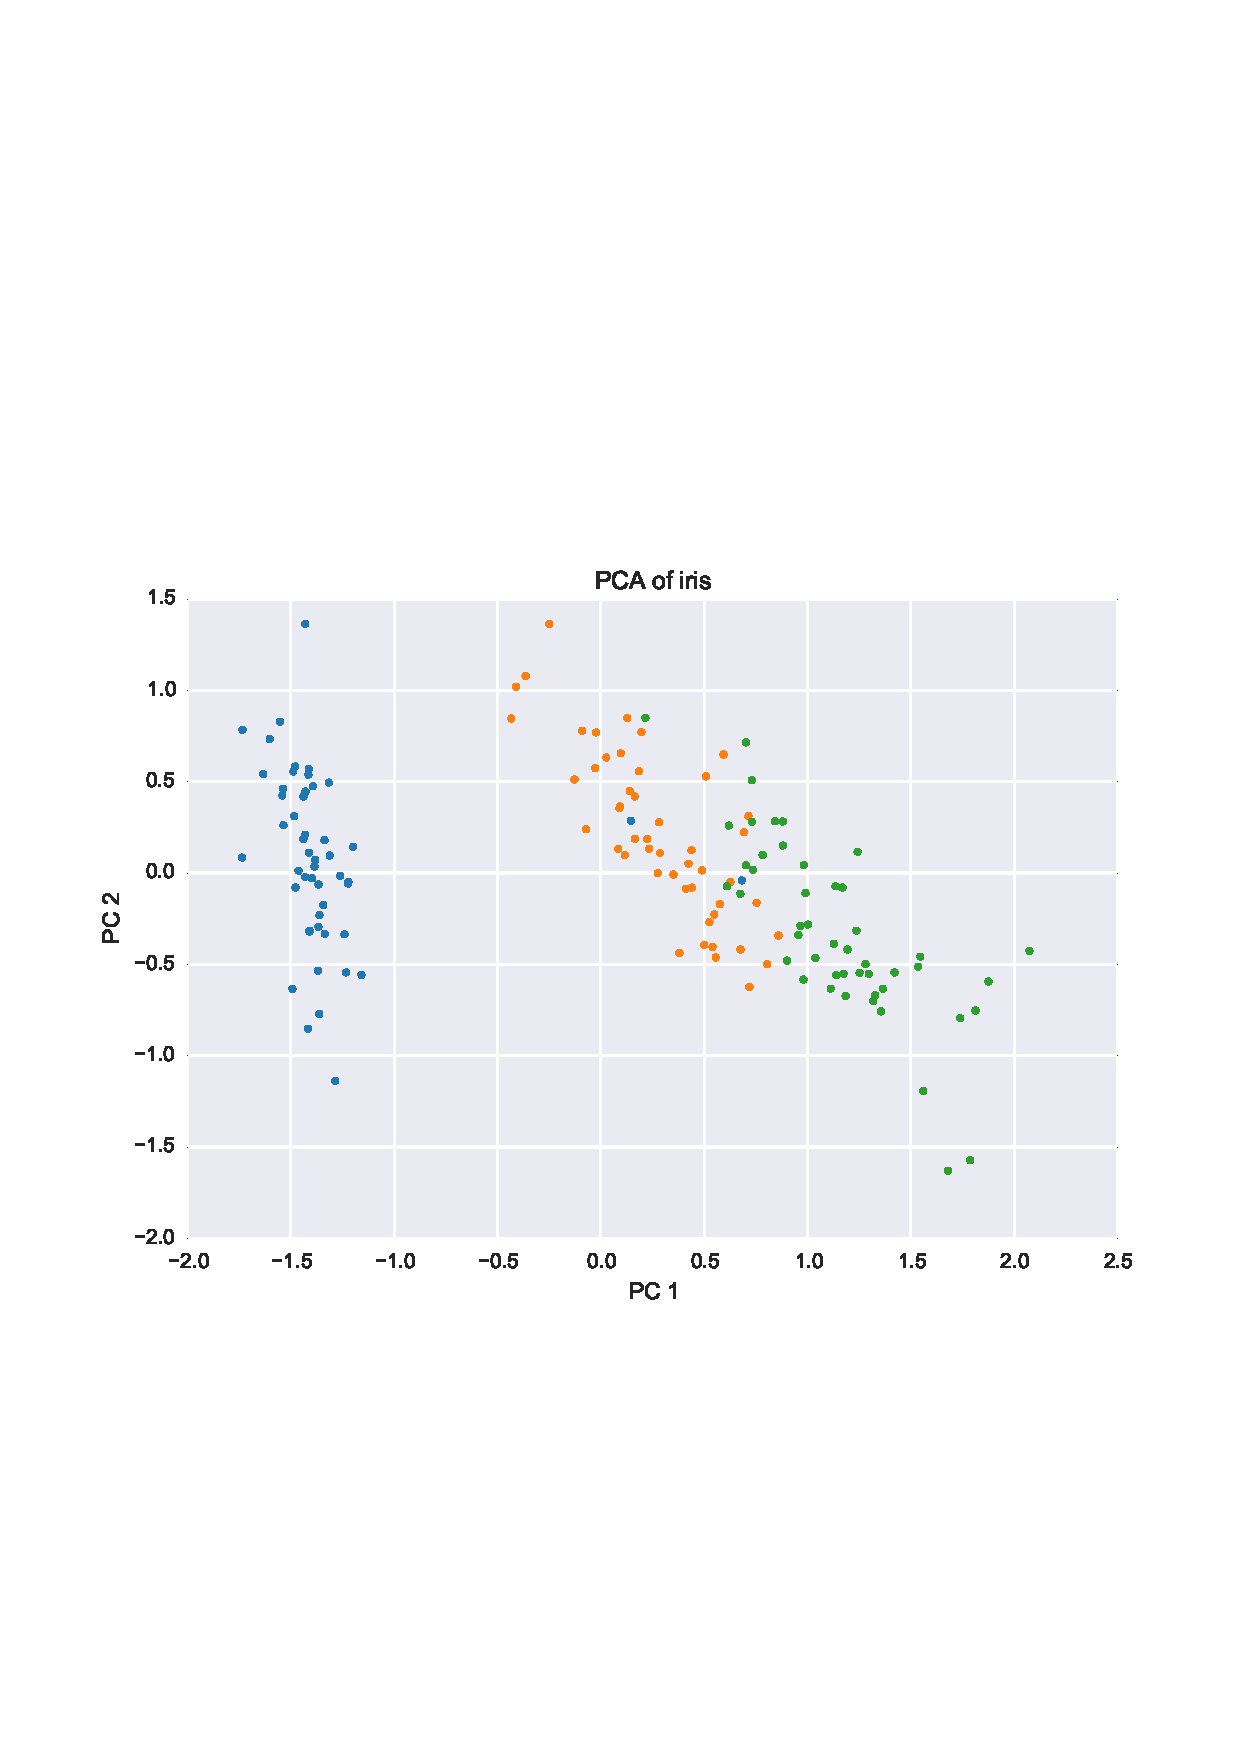
\includegraphics[scale=0.5]{Horn/img/iris_natural.png}
% \caption{Plot of the two first principal components (PC).}
% \label{fig:iris_natural}

% \end{figure}

% I chose $\sigma=\frac{1}{4}$ to reproduce the experiments in [3]. Only the first two PC are used here, which account for $95.8\%$ of the energy. The clustering results can be seen in Fig. \ref{fig:iris_2pc_cluster} and have an accuracy of 86\% computed with consistency index.


% \begin{figure}[hbtp]
% \centering
% 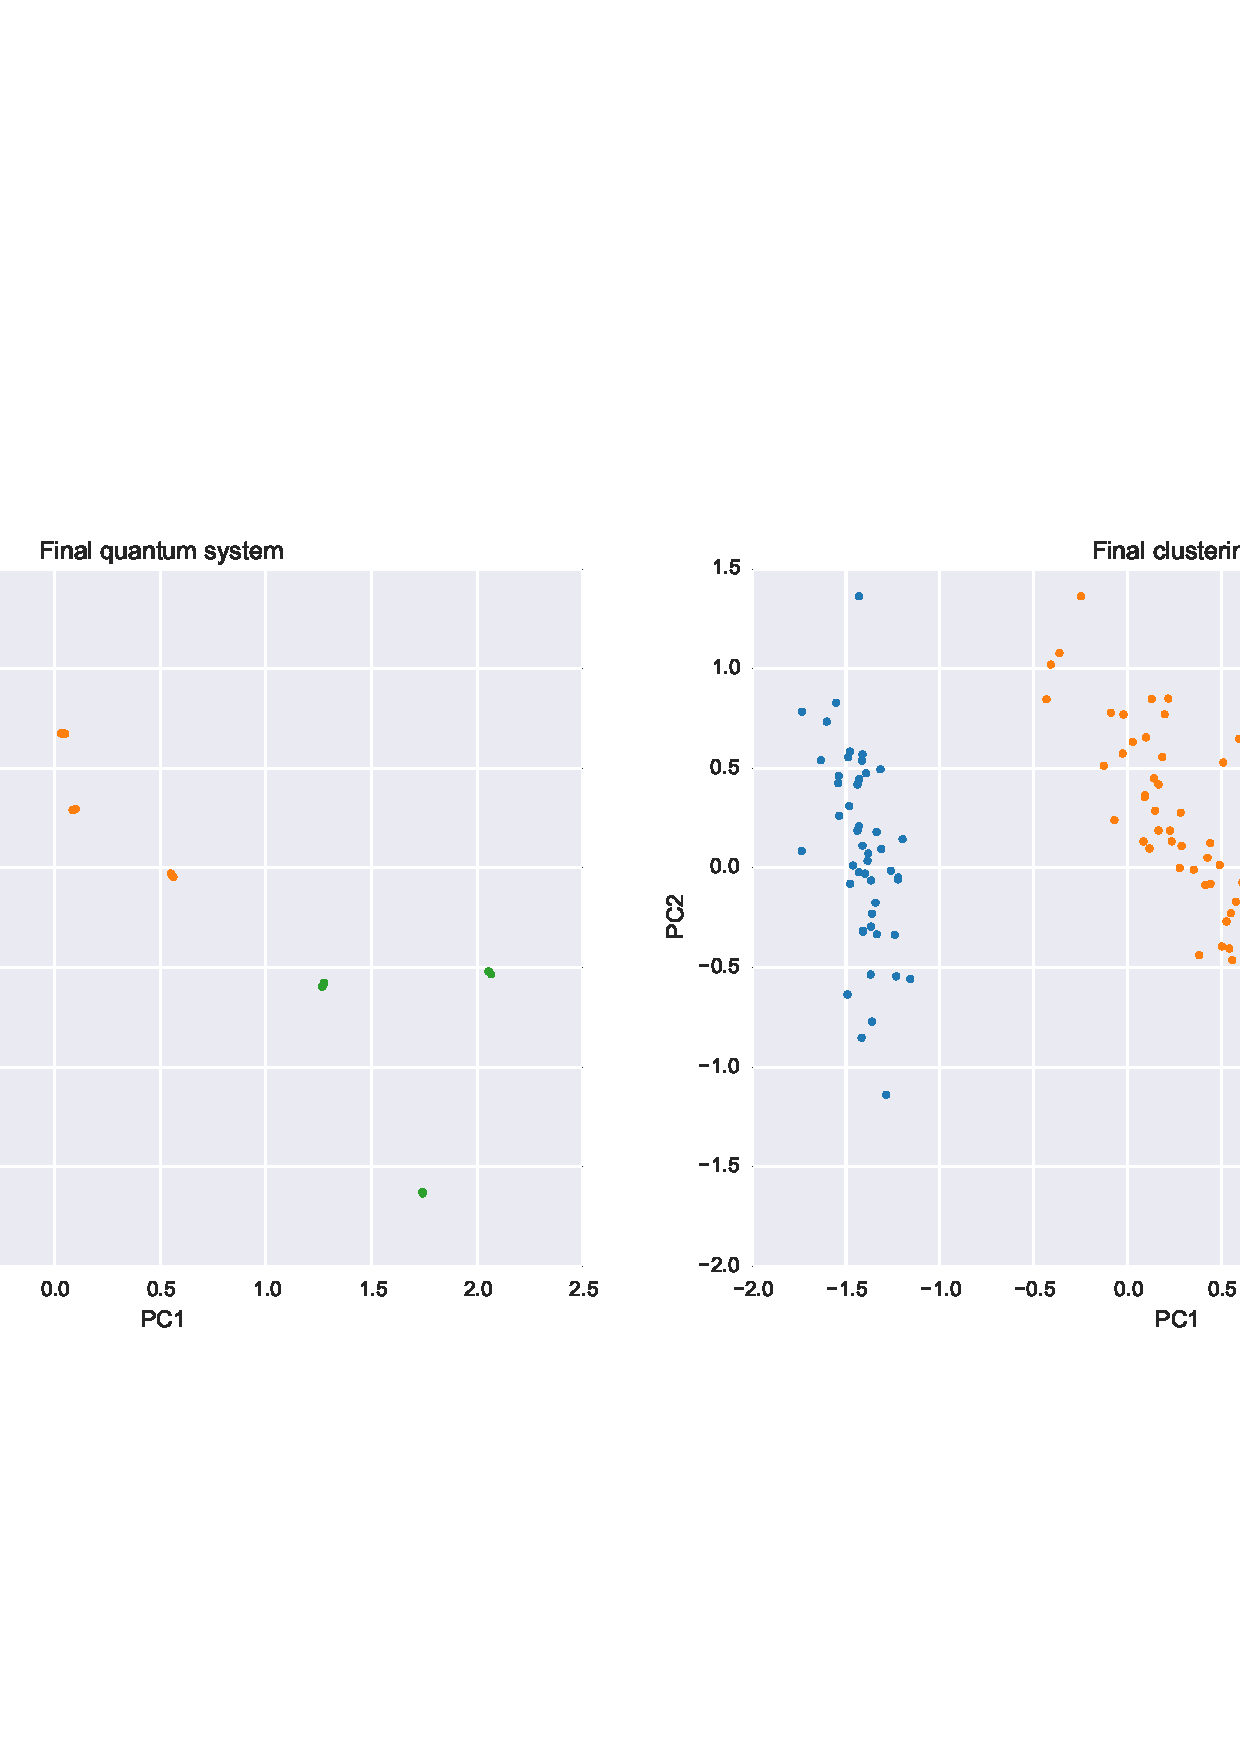
\includegraphics[width=\textwidth]{Horn/img/iris_2pc_cluster.png}
% \caption{Plots of the converged data data points and final clustering for 2 PC.}
% \label{fig:iris_2pc_cluster}

% \end{figure}

% For the sake of completeness, Fig. \ref{fig:iris_allpc_cluster} shows the clustering over all PCs. This solution has an accuracy of 82.67\% computed with consistency index.


% \begin{figure}[hbtp]
% \centering
% 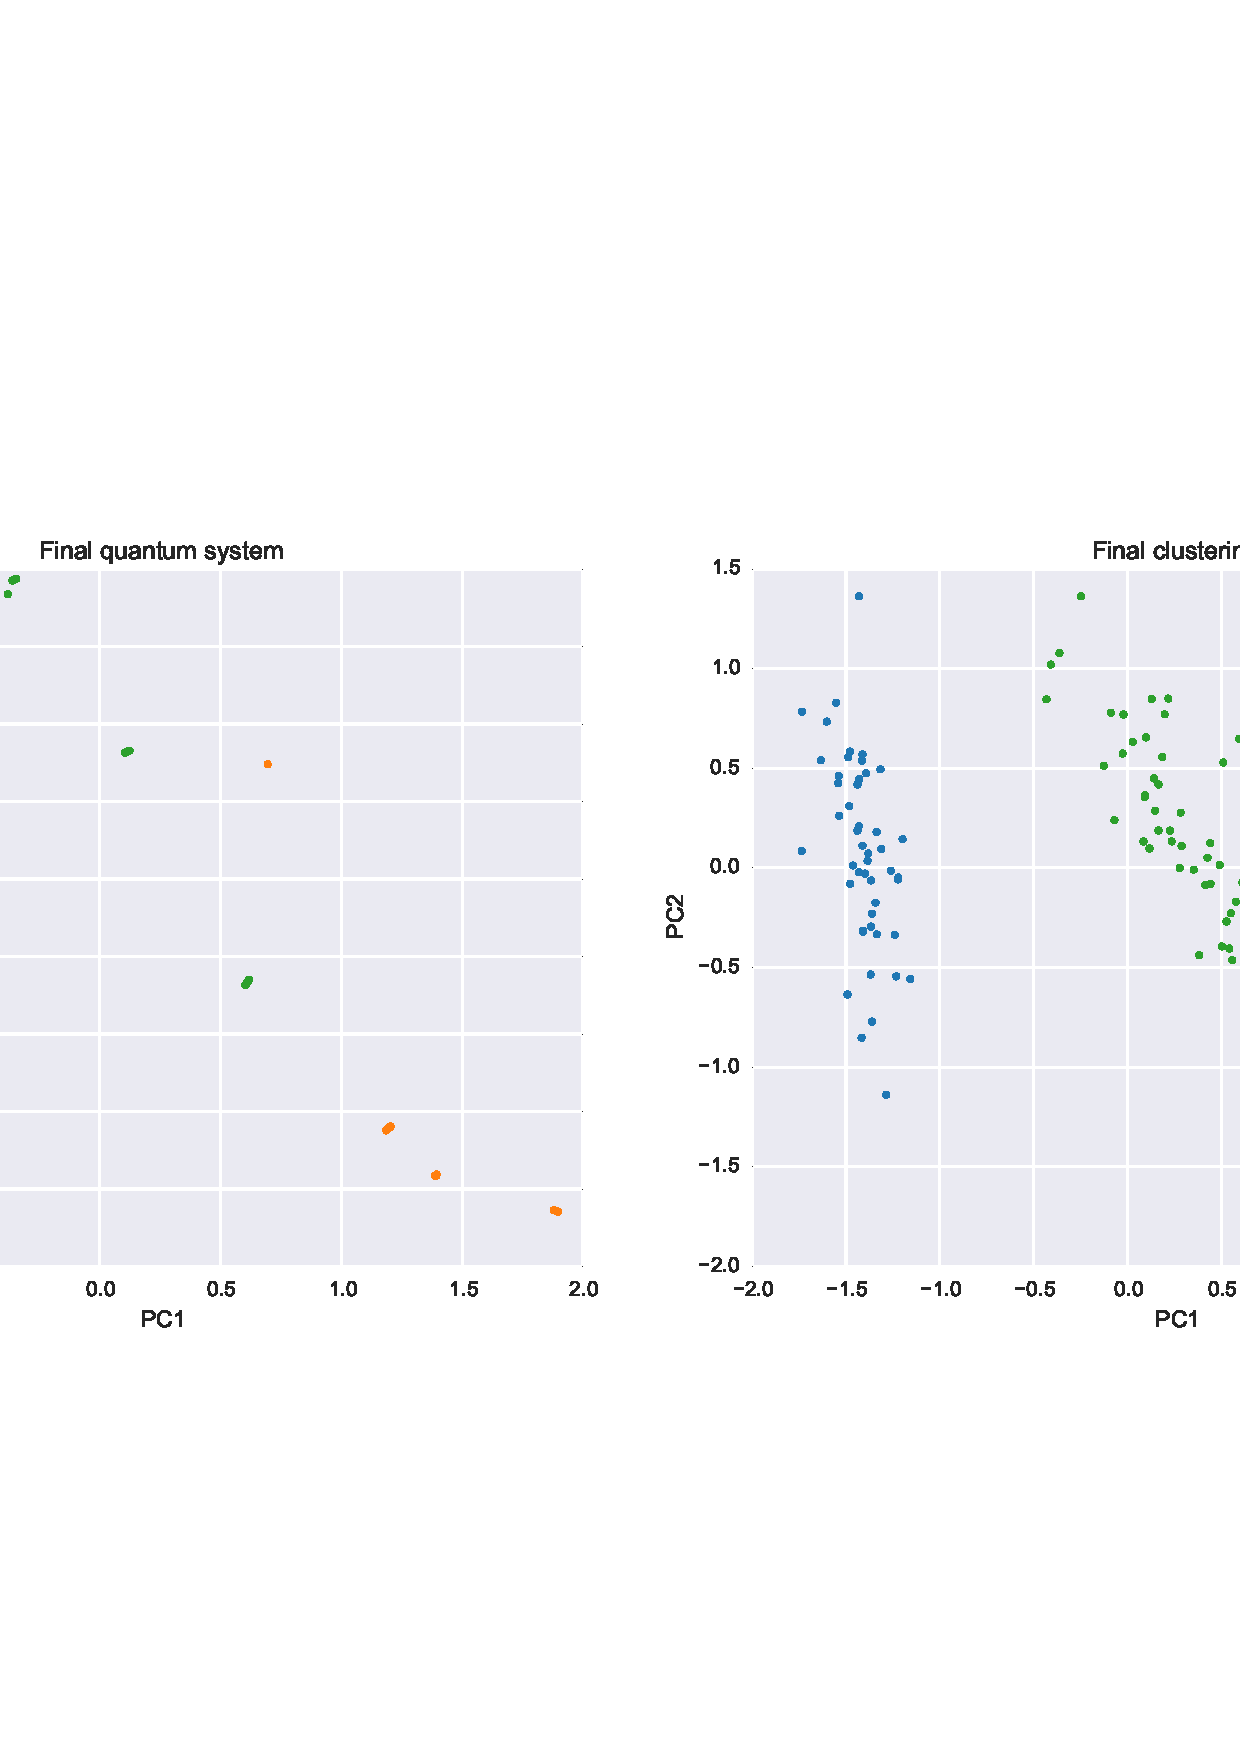
\includegraphics[width=\textwidth]{Horn/img/iris_allpc_cluster.png}
% \caption{Plots of the converged data data points and final clustering for all PC of Iris data.}
% \label{fig:iris_allpc_cluster}
% \end{figure}


% \subsection{Crab data}

% The crabs dataset has 200 samples and describes 5 morphological measurements on 50 crabs each of two colour forms and both sexes (total of 200 crabs), of the species Leptograpsus variegatus collected at Fremantle, Western Australia. After a preprocessing using PCA with covariance matrix and uncentred data, the dataset is represented in Fig. \ref{fig:crab_2pc_covar}.% #TODO add reference to dataset -->

% \begin{figure}[hbtp]
% \centering
% 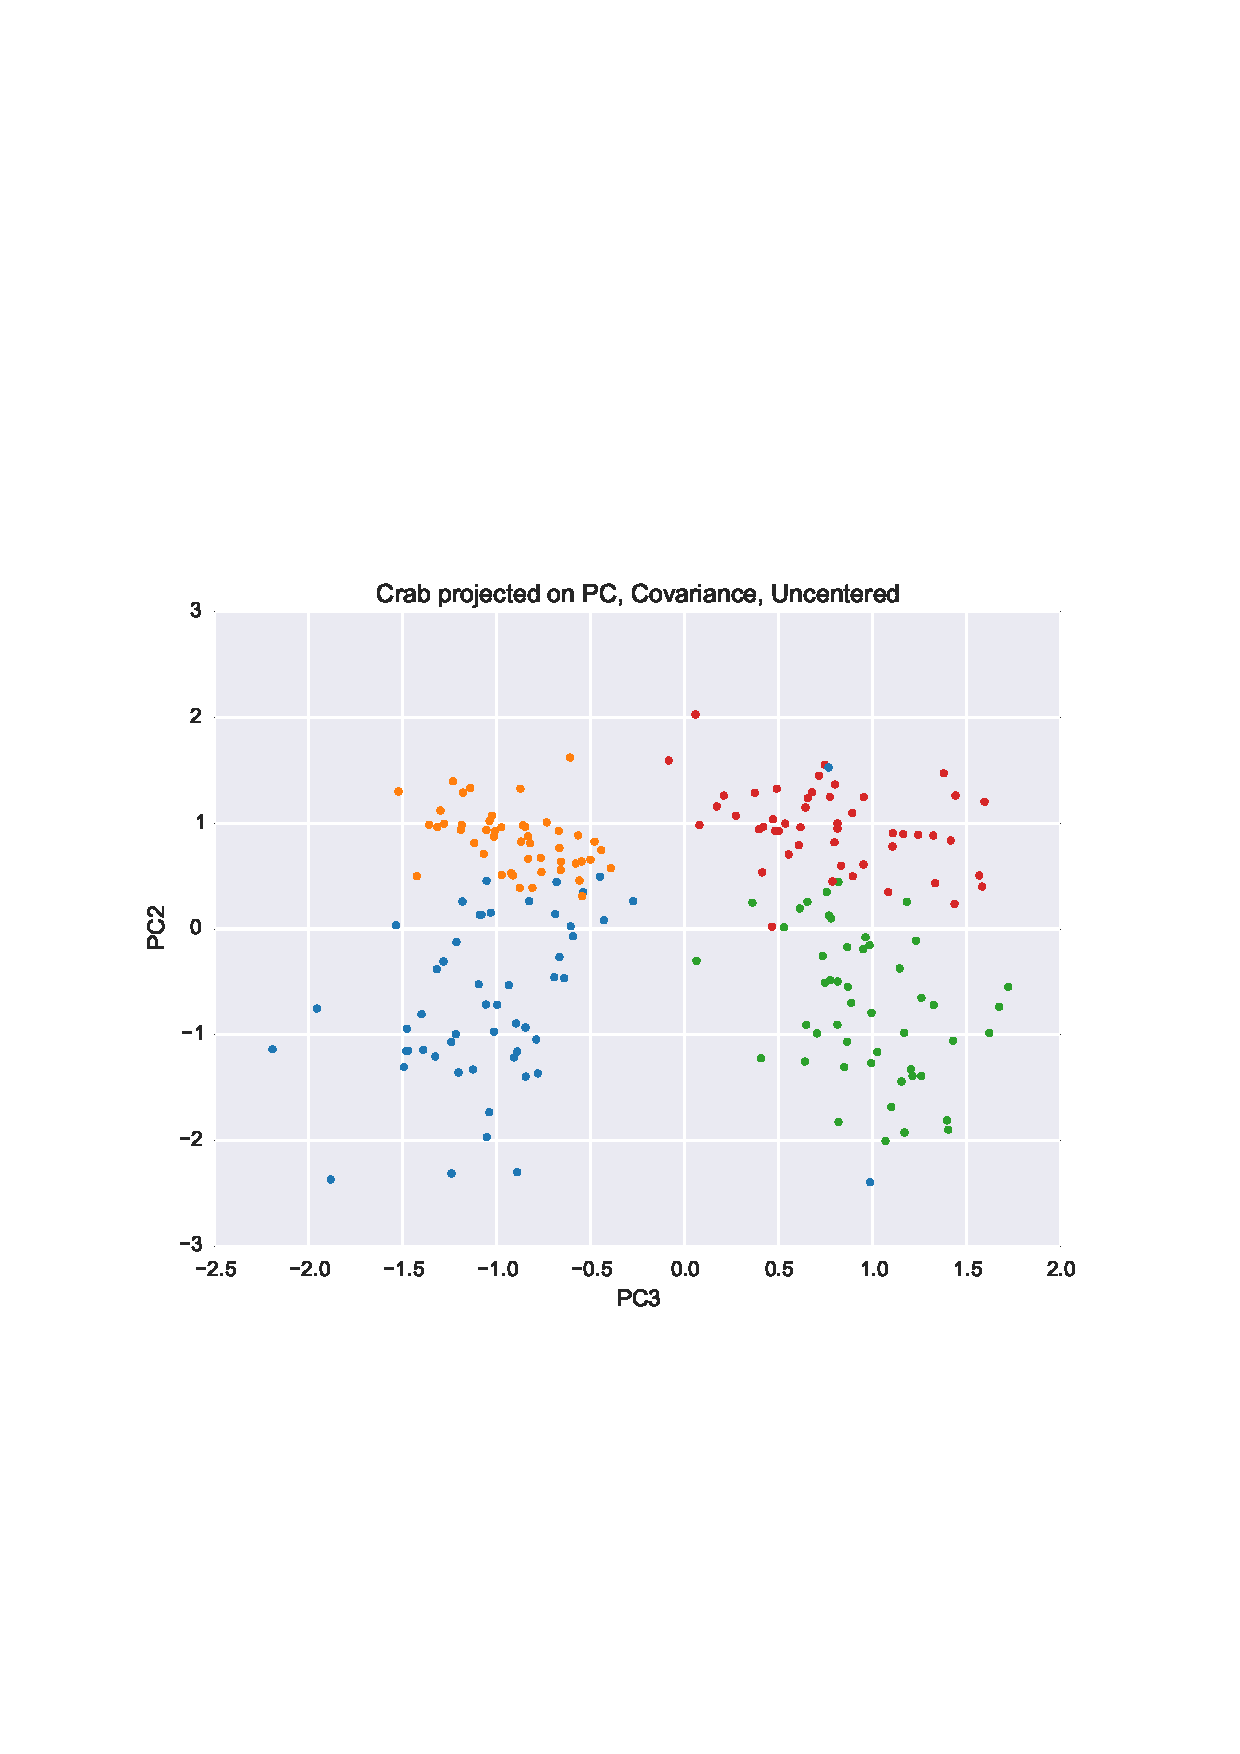
\includegraphics[scale=0.5]{Horn/img/crab_2pc_covar.png}
% \caption{Representation of the crab data projected over PC 2 and 3.}
% \label{fig:crab_2pc_covar}
% \end{figure}

% \begin{figure}[hbtp]
% \centering
% 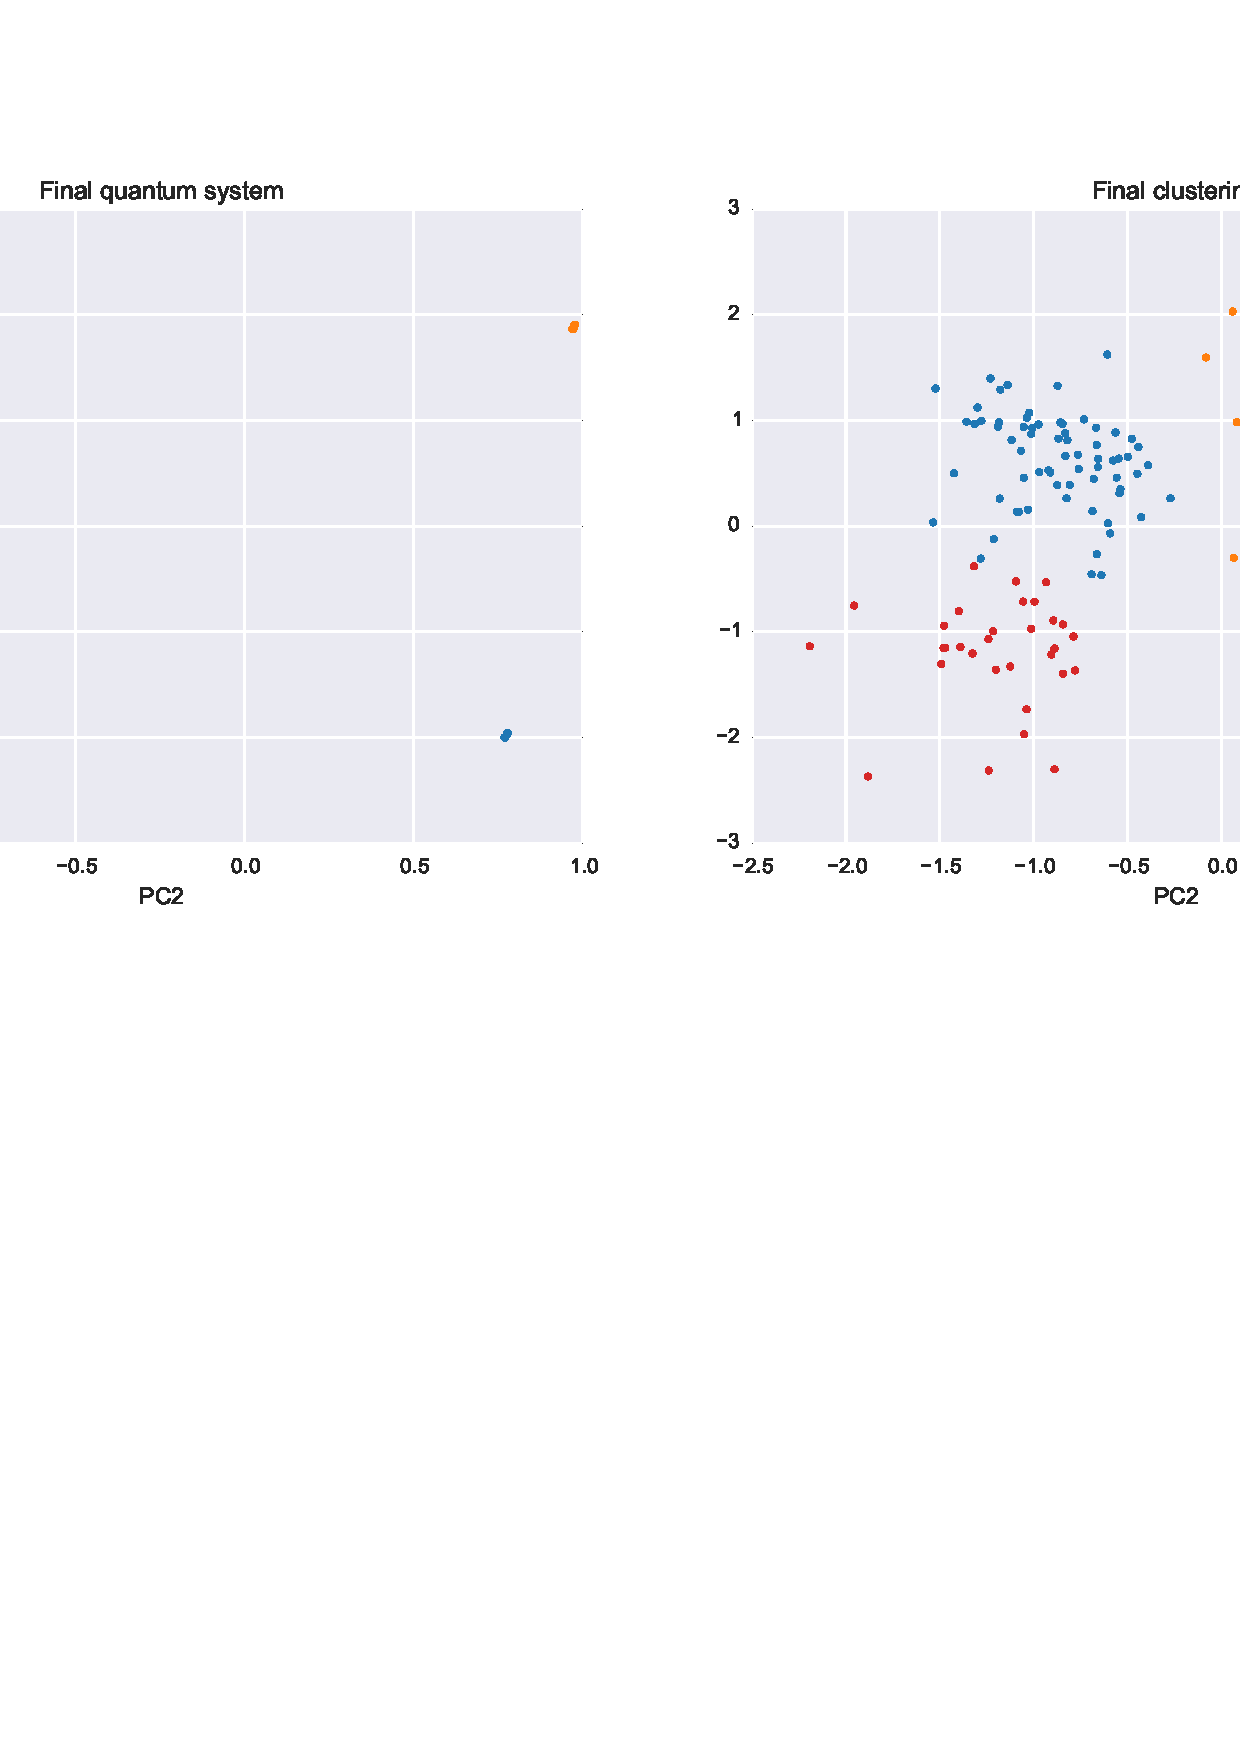
\includegraphics[width=\textwidth]{Horn/img/crab_2pc_covar_cluster.png}
% \caption{Representation of the crab data projected over PC 2 and 3.}
% \label{fig:crab_2pc_covar_cluster}
% \end{figure}

% \begin{figure}[hbtp]
% \centering
% 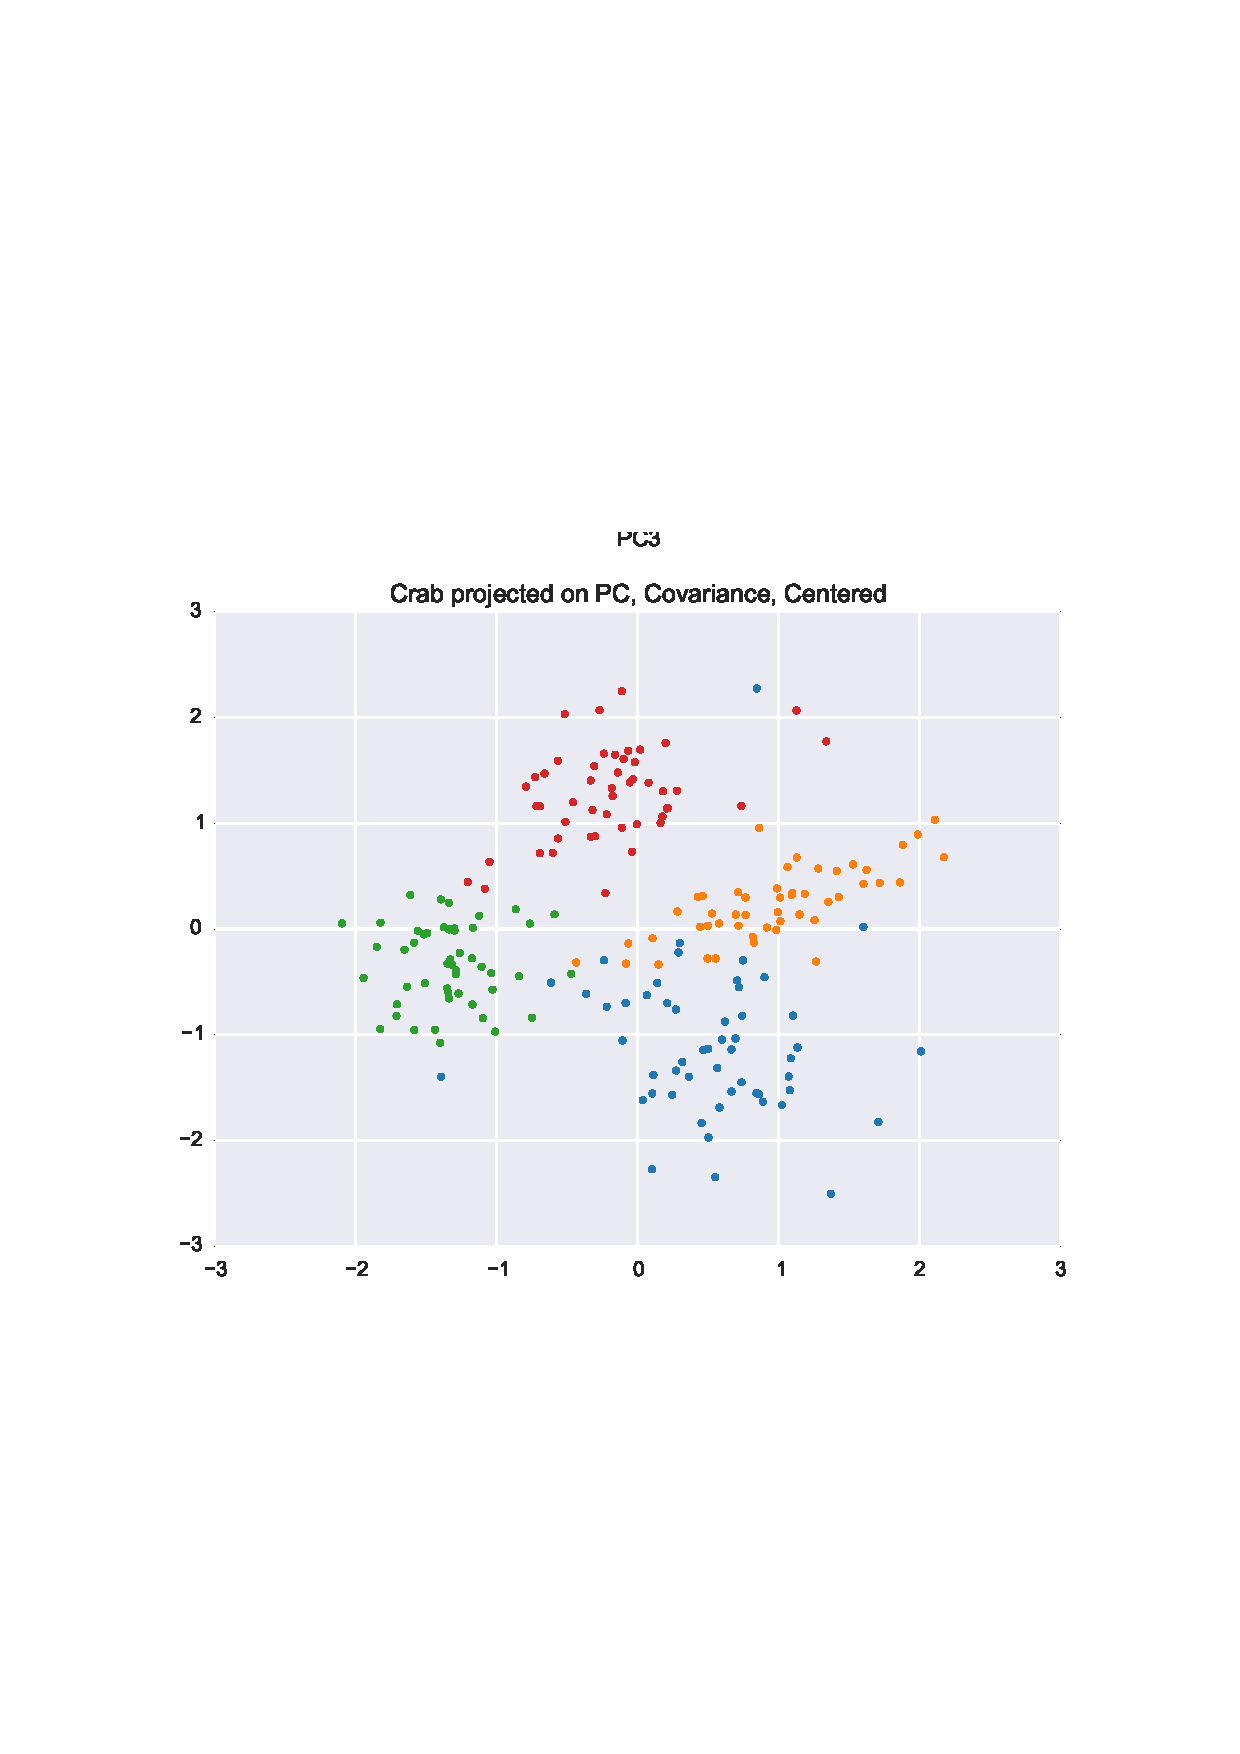
\includegraphics[scale=0.5]{Horn/img/crab_2pc_covar_centered.png}
% \caption{Representation of the crab data projected over PC 2 and 3.}
% \label{fig:crab_2pc_covar_centered}
% \end{figure}

% \begin{figure}[hbtp]
% \centering
% 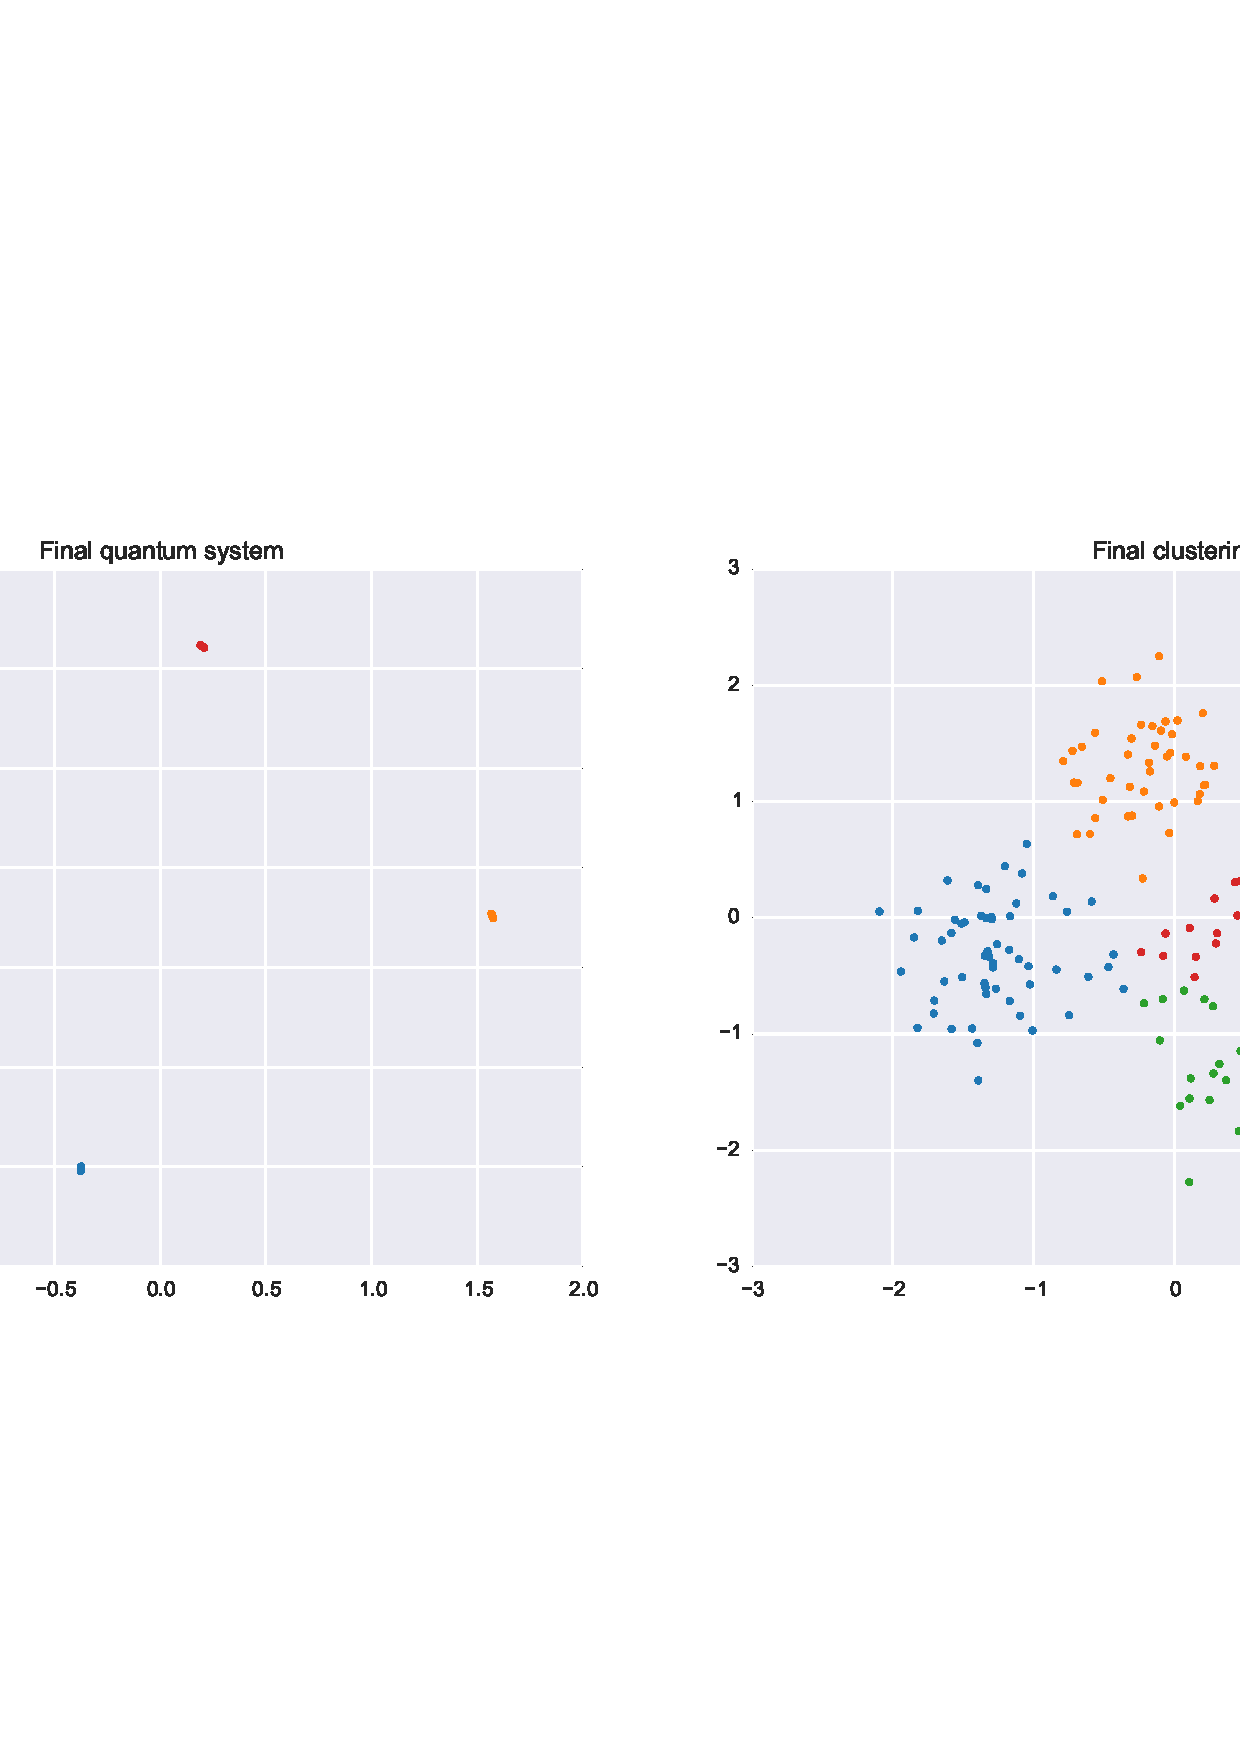
\includegraphics[width=\textwidth]{Horn/img/crab_2pc_covar_centered_cluster.png}
% \caption{Representation of the crab data projected over PC 2 and 3.}
% \label{fig:crab_2pc_covar_centered_cluster}
% \end{figure}


% Initial work aimed at reproducing results from [2], but lack of detail on the preprocessing used made it an harder task. Several preprocessings were used, namely whitening or not the data, centring it or not, using covariance versus correlation and different methods of computing the PCs through eigenvalue decomposition or Singular Value Decomposition (SVD). The closest representation to that of the [2] is the one if Fig. C1.


% %TODO finish crab

% Covariance uncentred consistency index = 0.815
% Covariance centred consistency index = 0.91

% all pc covariance uncentred consistency index = 0.63
% all dimensions original data consistency index = 0.34

%--------------------------------------------%
%--------------------------------------------%
%             CONCLUSIONS
%--------------------------------------------%
%--------------------------------------------%

\section{Conclusion}

% \subsection{Conclusions}
\begin{frame}{Conclusions}
\begin{itemize}
\item Lessons learned: time vs. memory efficiency
\item GPU is a valuable and widely widely available resource for data processing
\item EAC was successfully scaled:
	\begin{itemize}
	\item GPU K-Means
	\item Efficient sparse matrix building
	\item MST equivalence with SL
	\item Disk-based algorithms
	\end{itemize}

\item Contributions:
	\begin{itemize}
	\item Widen the range of EAC's applicability 
	\item New of way of building sparse matrix
	\item New $K_{min}$ rules for sparsity optimizations
	\end{itemize}

\item Plenty of possible extensions

\item Selected parts of this work was compiled and submitted as a conference article

\end{itemize}
\end{frame}

% \subsection{References}
%   \begin{frame}{References}
%       \printbibliography
%   \end{frame}


% blank side for ending
\bgroup
\setbeamercolor{background canvas}{bg=black}
\begin{frame}[plain]{}
\end{frame}
\egroup

\end{document}